\section{Time and Frequency Synchronization}
\subsection{The Problem of Synchronization}
It is important that the transmitter and receiver are synchronized in order for the demodulation to be accurate. The receiver must precisely determine when to sample the incoming complex signal to capture the symbol values and align its local carrier frequency and phase with that of the received signal. \par
Physically, synchronization errors occur when the transmitter and receiver operate with independent local oscillator. The local oscillators can be subject to manufacturing imperfection, environmental variation, leading to slight deviations from their target frequencies. Furthermore, the propagation delay of the signal between the transmitter and the receiver introduces an unknown phase shift in the carrier and an unknown time shift in the symbol sequence arrival.\par
These phenomena give rise to four types of synchronization errors, which can be categorized into carrier synchronization errors and timing synchronization errors.
\begin{itemize}
	\item Carrier Frequency Offset (CFO): $\Delta_f$, which is the difference in carrier frequency between the transmitted symbols and the received symbols
	\item Carrier Phase Offset $\phi_0$: phase difference between the transmitted symbols and the received symbols
	\item Sample Clock Offset (SCO): $\delta$. This error occurs when the frequency of the clock driving the Analog-to-Digital Converter at the receiver differs from that of the Digital-to-Analog Converter at the transmitter	. This error type was not implemented in the project and was considered negligible.
	\item Time shift: $t_0$, represents the receiver's uncertainty about the exact time of arrival of the symbols. The receiver needs to determine the optimal sampling instants, which correspond to the peaks of the Nyquist-filtered pulses.
\end{itemize}

Figure \ref{fig:sync-errors-conceptual} illustrates these mismatches. The transmitter generates symbols at discrete times $nT_{symb}$; which are then pulse-shaped and modulated. At the receiver, after down-sampling, the signal is sampled at instances $nT_{symb}(1+\delta)+t_0$ relative to the transmitter.
\begin{figure}[H]
	\centering
	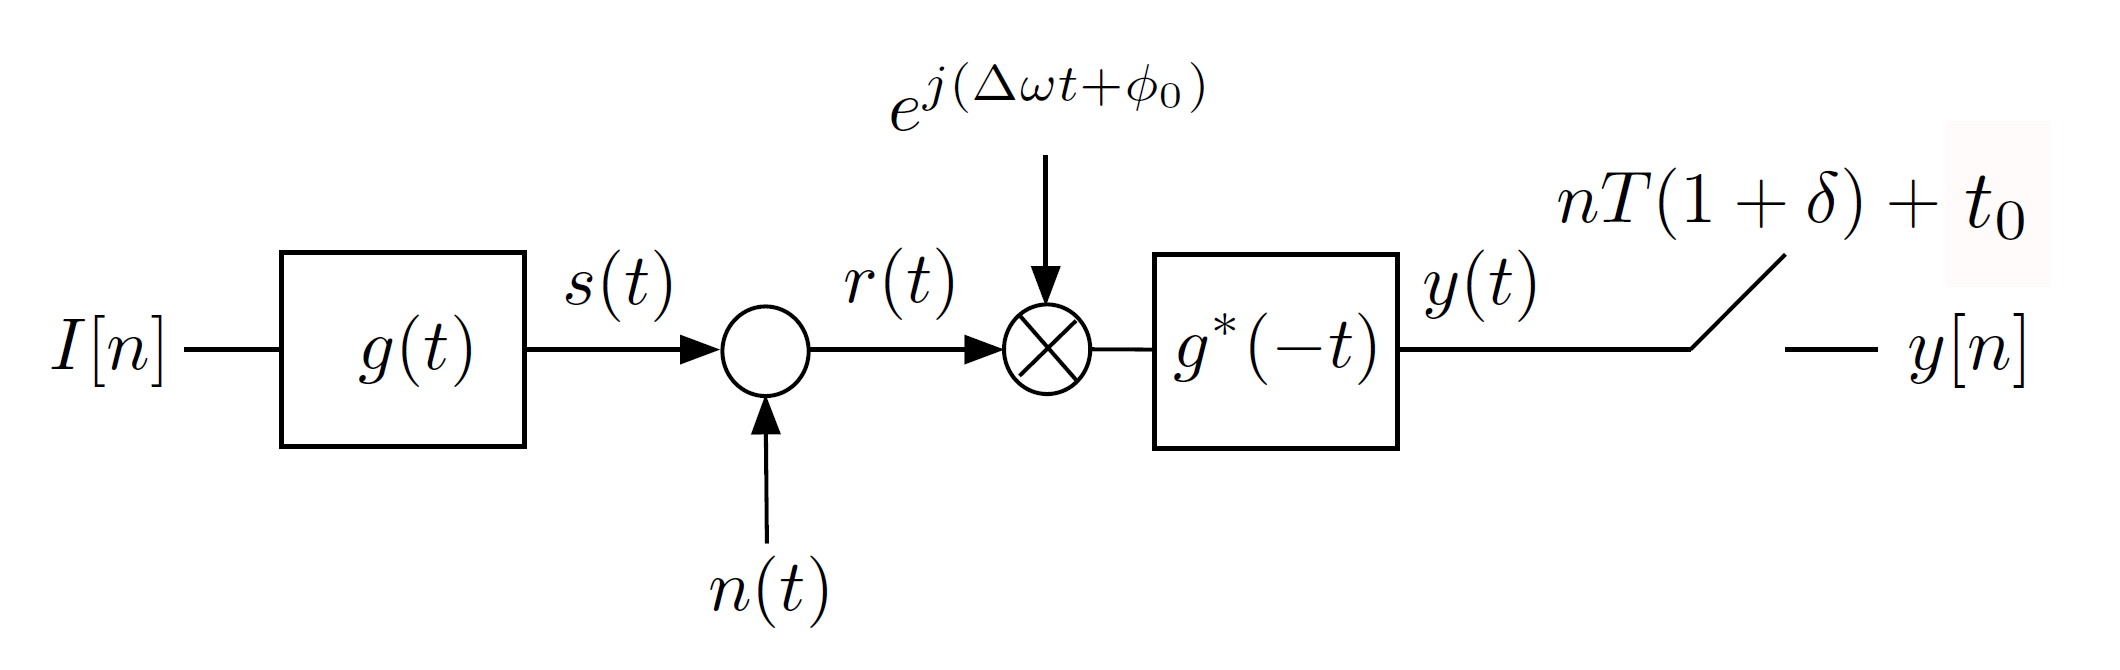
\includegraphics[width=0.8\linewidth]{Images/sync-errors-conceptual}
	\caption{Synchronization mismatches at the receiver}
	\label{fig:sync-errors-conceptual}
\end{figure}

\subsection{Impact of Synchronization Errors on Performance}
\subsubsection{Impact of Carrier Phase Offset ($\phi_0$)}
A static carrier phase offset arises from the unknown phase difference between the incoming carrier signal and the receiver local oscillator. Assuming perfect timing and no CFO, if the transmitted complex baseband symbol is $I[n]$, the corresponding sample y[n] at the output of the matched filter becomes:
\begin{equation}
	y[n] = I[n]e^{j\phi_0} + \text{noise}
\end{equation}
this equation shows that the phase offset causes a rotation of the entire received symbol constellation by an angle $\phi_0$ in the complex plane.
Figure \ref{const-errors} illustrate a constellation diagram before and after applying a phase offset.
\subsubsection{Impact of Carrier Frequency Offset}
If $r(t)$ is the signal before the matched filter, then it becomes $r(t) e^{j(2\pi \Delta f t + \phi_0)} + \text{noise}$, where $\phi_0$ is the initial phase offset.\par
The impacts of CFO are therefore:
\begin{enumerate}
	\item Phase Drift: After matched filtering and sampling at $t = nT_{symb}$, each symbol $I[n]$ experiences a phase rotation that changes from symbol to symbol: $y[n] = I[n] e^{j(2\pi \Delta f t + \phi_0)} + \text{noise}$. Figure \ref{const-errors} shows the received symbol after CFO as a spiral pattern, due to the progressive phase rotation.
	\item Inter-Symbol Interference: If the CFO is significant, the assumption that it only causes a phase rotation at the matched filter output is no longer accurate. The term $e^{2\pi \Delta f t}$ means that the received signal spectrum is shifted. The matched filter $g^*(-t)$ is no longer matched to the incoming because signal $g'(t) = g(t) e^{2\pi \Delta f t}$, leading to ISI.
\end{enumerate}
\subsection{Impact of Sample Time Shift}
An incorrect sampling instant means that the output of the matched filter is not sampled at the point of maximum signal energy and zero ISI. if $h(t)$ is the impulse response of the overal Nyquist filter (Raised Cosine Filter), and sampling occurs at $nT_{symb} + t_0$, the $n$-th sample $y[n]$ is given by:
\begin{align}
	y[n] = \sum_m I[m]h((n-m)T_{symb} + t_0) + \text{noie}\\
	y[n] = I[n]h(t_0) + \sum_{m \neq n} I[m]h((n-m)T_{symb} + t_0) + \text{noise}
\end{align}
The first term $I[n]h(t_0)$, represents the desired symbol and the secon term is the ISI, arising because $h(hT_{symb} + t_0)$ is non-zero for $k \neq 0$ when $t_0 \neq 0$
\subsection{Gardner Algorithm for Sampling Time Tracking}
\subsection{Frame and Frequency Acquisition using Differential Cross-Correlator}
\subsection{Phase Interpolation}
\subsection{Questions and Answers}